\chapter{Research Methodology} \label{chp:method}

This chapter will cover the methodology employed to develop the grey box model. The grey box modelling approach adopted in this thesis falls within the category of sequential GBM. Consequently, the development process is divided into two stages. The initial stage of the modelling process focuses on machine learning, specifically the development of the BBM using tree-based models. This is carried out using Python in conjunction with \scikit/ \bcitep{FabianPedregosa.2011}. This stage encompasses data acquisition, data preprocessing, hyperparameter optimization, and model evaluation. The training of the models involves a fusion of T-AIS data and weather data, followed by the selection of relevant features for predicting the SOG. These processes are visually illustrated in \Cref{fig:flowchart_BBM}.

\begin{figure}[h]
    \centering
        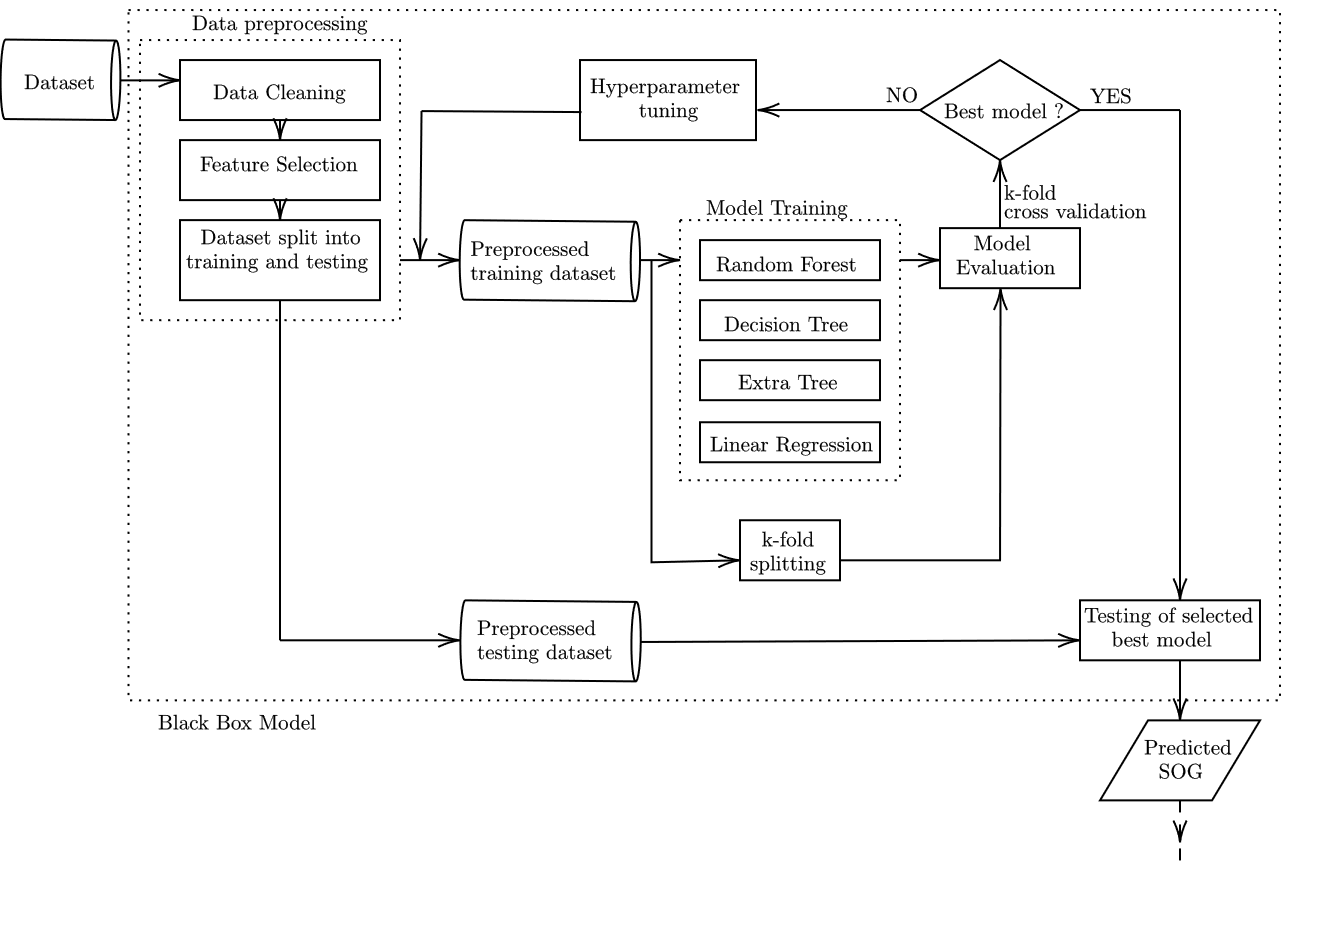
\includegraphics[width=\textwidth]{02_figures/flowmethod_BBM_alt.png}
        \caption{Scheme of proposed BBM methodology}
        \label{fig:flowchart_BBM}
\end{figure}

The second stage of the modelling process is centred around the WBM component of the GBM. In this phase, the predicted SOG serves as input for the WBM to forecast the necessary brake power required for propelling the ship. This involves an initial conversion of SOG to STW for estimation of encountered resistance during the voyage, this then facilitates the estimation of the required power i.e. energy required to propel the ship. The framework outlined in \Cref{fig:flowchart_WBM} provides a graphical depiction summarising the concepts discussed in \Cref{sec:power_calc}.

\begin{figure}[h]
    \centering
        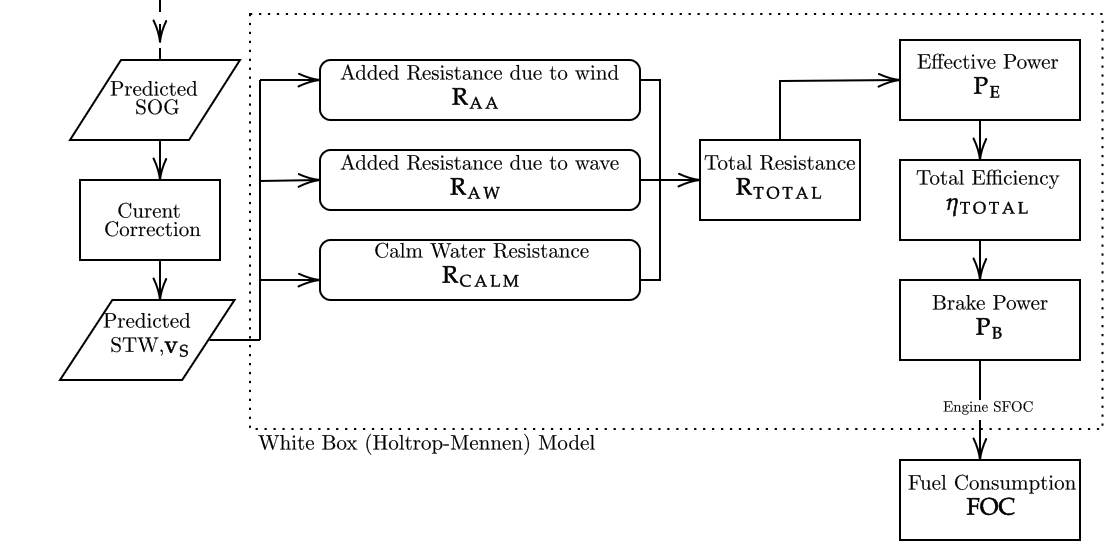
\includegraphics[width=\textwidth]{02_figures/flowmethod_WBM.png}
        \caption{Scheme of proposed WBM methodology adopted from \bcitet{XiaoLang.2020}}
        \label{fig:flowchart_WBM}
\end{figure}

The development process of GBM is summarised in \Cref{fig:flowchart_GBM}. Detailed discussion regarding the development of BBM and WBM model will be discussed in the following sections of this chapter.

\begin{figure}[h]
    \centering
        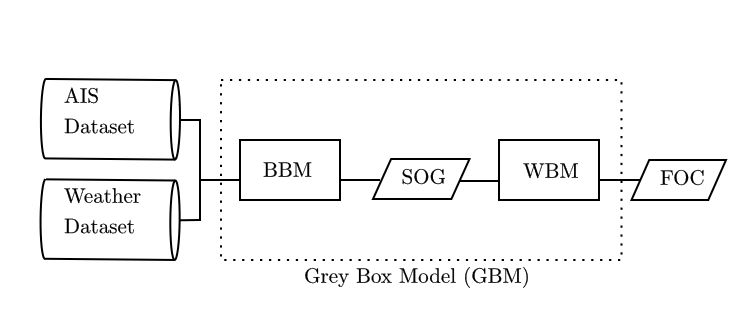
\includegraphics[width=.85\textwidth]{02_figures/flowmethod_GBM_alt.png}
        \caption{Scheme of proposed GBM methodology}
        \label{fig:flowchart_GBM}
\end{figure}

\pagebreak

\section{Data Acquisition}\label{sec:data_acquisition}

The data is collected from a ferry serving between ports of K{\o}ge, R{\o}nne, Ystad and Sassnitz, as shown in \Cref{fig:Hammershus_journey_map} \bcitep{HammershusJourney}. The trip between K{\o}ge, R{\o}nne takes about 5 h 30 minutes and it sails between R{\o}nne and Sassnitz for 3 h and 20 minutes. The journey is tracked by the T-AIS system of the Danish Maritime Authority (DMA). The weather data along her sailing path are acquired from ECMWF\footnote{European Centre for Medium-Range Weather Forecast} with a temporal resolution of 1 hour at a spatial granularity of 0.25° (longitude) x 0.25° (latitude), data from ECMWF provides information for wind, waves and seawater temperature. The information for current is obtained from CMEMS\footnote{Copernicus Marine Environment Monitoring Service} with a temporal resolution of 3 hours at a spatial granularity of  0.25° (longitude) x 0.25° (latitude).\\ 

\begin{figure}[ht]
  \begin{minipage}{0.55\linewidth} % Adjust the width as needed
    \footnotesize
    \centering
    \begin{tabular}{l r}
        \hline
        IMO & 9812107 \\
        Type \& Service & Passenger ferry \\
        $L_{OA}$ & 158.00 m\\
        $L_{WL}$ & 144.80 m\\
        $B$ (moulded) & 24.5 m\\
        $T_{DESIGN}$ & 5.70 m\\
        $T_{MAX}$ & 5.85 m \\ 
        Gross Tonnage (GT) & 18,009 \\
        Deadweight (dwt) & 4,830 t \\
        Main Engines & Wärtsillä 8V31 2 x 4,880 kW \\
        SFOC & 169.4 g/kWh \\
        Service Speed & 17.7 knots \\
        Bow Thrusters & 2 x 1500 kW \\
        \hline
    \end{tabular}
    \caption{Particular of M/S Hammershus}
    \label{tbl:Hammershus_Data}
  \end{minipage}
  \hspace{0.01\linewidth}
%   \hfill
  \begin{minipage}{0.43\linewidth} % Adjust the width as needed
    \centering
    % \vspace*{0.1cm}
    \includegraphics[width=\linewidth]{02_figures/Bornholmerfærgen_route_map.png} % Replace example-image.jpg with your picture file name
    \caption{Journey of the ferry}
    \label{fig:Hammershus_journey_map}
  \end{minipage}
\end{figure}


\begin{figure}[h]
    \centering
        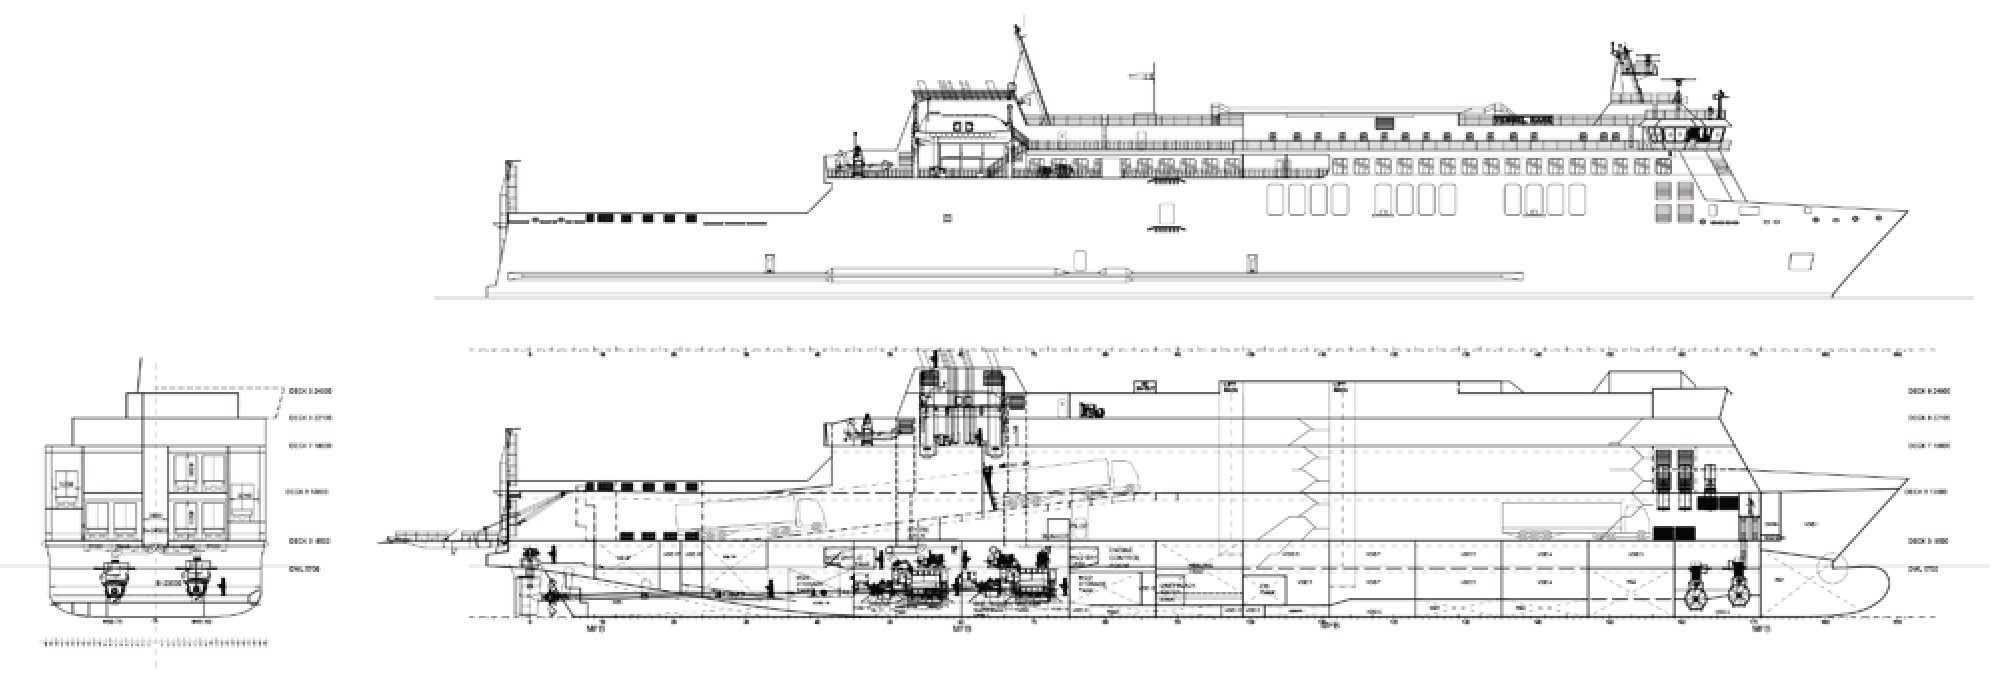
\includegraphics[width=\textwidth]{02_figures/Hammershus_Pict.jpg}
        \caption{Schematics of M/S Hammershus}
        \label{fig:Hammershus_Pict}
\end{figure}

The resulting combined dataset maintains a temporal resolution of 1 hour. To address the disparity between the temporal resolutions of the data from CMEMS and ECMWF, the weather information is synchronised. This synchronisation ensures that the wind, waves, seawater temperature, and sea current data align with the same weather grid and possess consistent temporal resolutions. The features \textbf{wind direction},\textbf{swell direction}, and \textbf{wind wave direction} are oriented to true north. However, to reflect the actual direction of weather effects that are acting on the ship, these features are converted to true direction; where true direction is defined as the direction of weather effect with respect to the bow of the ship. The value ranges between 0° and 180°. Subsequently, through vector decomposition, the northward and eastward wind velocity is converted to absolute wind speed and wind direction \emph{with respect to True North},$\varphi$:

\begin{equation}\label{eqn:vwindabs}
    u_{\text{W}} = \sqrt{(u_{\text{W}_{N}})^2 + (u_{\text{W}_{E}})^2} 
\end{equation}
\begin{equation}\label{eqn:winddir}
    \varphi = 
    \begin{cases}
        360 - \arctan(u_{\text{W}_{E}} / u_{\text{W}_{N}}) \quad \text{\textbf{if}} \quad u_{\text{W}_{E}} > 0 \quad \wedge \quad u_{\text{W}_{N}} < 0 \\ 
        180 - \arctan(u_{\text{W}_{E}} / u_{\text{W}_{N}}) \quad \text{\textbf{if}} \quad u_{\text{W}_{E}} < 0 \quad \wedge \quad u_{\text{W}_{N}} > 0 \\ 
        270 - \arctan(u_{\text{W}_{E}} / u_{\text{W}_{N}}) \quad \text{\textbf{if}} \quad u_{\text{W}_{E}} > 0 \quad \wedge \quad u_{\text{W}_{N}} > 0 \\
        \arctan(u_{\text{W}_{E}} / u_{\text{W}_{N}}) \qquad \text{\textbf{otherwise}} 
    \end{cases}   
\end{equation}

Similarly, information of Northward and Eastward current Velocity is converted to the absolute current speed and current direction \emph{with respect to True North} $\gamma$.\\ 

\begin{equation}\label{eqn:vcurrabs}
    v_{\text{C}} = \sqrt{(v_{\text{C}_N})^2 + (v_{\text{C}_E})^2} 
\end{equation}
\begin{equation}\label{eqn:currdir}
    \gamma = 
    \begin{cases}
        360 - \arctan(u_{\text{W}_{E}} / u_{\text{W}_{N}}) \quad \text{\textbf{if}} \quad v_{\text{C}_E} < 0 \quad \wedge \quad v_{\text{C}_N} > 0 \\ 
        180 - \arctan(u_{\text{W}_{E}} / u_{\text{W}_{N}}) \quad \text{\textbf{if}} \quad v_{\text{C}_E} > 0 \quad \wedge \quad v_{\text{C}_N} < 0 \\ 
        270 - \arctan(u_{\text{W}_{E}} / u_{\text{W}_{N}}) \quad \text{\textbf{if}} \quad v_{\text{C}_E} < 0 \quad \wedge \quad v_{\text{C}_N} < 0 \\
        \arctan(u_{\text{W}_{E}} / u_{\text{W}_{N}}) \qquad \text{\textbf{otherwise}} 
    \end{cases}   
\end{equation}

The initial dataset offers data in true directions, indicating the direction in which weather conditions are encountered relative to the ship's bow. The static information from AIS data, which includes the ship's identity and navigational status, is excluded from the dataset. The original structure encompasses 27 features: 9 AIS features and 18 weather features. The layout of the initial dataset, prior to data preprocessing and feature selection, is outlined in Table \Cref{tbl:dataset_init_struct}.

\begin{table}[h!]
    \footnotesize
    \centering
    % \resizebox {\textwidth}{!}
    {\begin{tabular}{ p{0.4\textwidth} c }
    \hline
    \textbf{Feature} & \textbf{Feature Name}  \\
    \hline
    \multicolumn{2}{l}{\textbf{AIS data}}\\
    \hline
    Position Time Stamp [DD\slash MM\slash YYYY HH:MM:SS] & {\tt Time} \\
    Latitude [°] & {\tt LAT}   \\
    Longitude [°] & {\tt LON}  \\
    Width [m] & {\tt width}  \\
    Length [m] & {\tt length}\\
    SOG [Knots] & {\tt sog} \\
    COG [m/s] & {\tt cog}  \\
    Heading [°] & {\tt heading}  \\
    Draught [m] & {\tt draught} \\
    \hline
    \multicolumn{2}{l}{\textbf{Weather Data (0.5° Granularity)}}\\
    \hline
    Wind Speed [m/s] & {\tt windspeed} \\
    True North Wind Direction, $\varphi$ [°] & {\tt truenorthcurrentdir} \\
    Air Temperature Above Oceans [K] & {\tt oceantemperature} \\
    % Air Density Above Oceans [$\text{kg/m}^3$]& - \\
    Maximum Wave Height [m] & {\tt waveheight} \\
    % Swell Direction [°] & - \\
    % Wind Wave Direction & - \\
    Swell Period [s] & {\tt swellperiod} \\
    Wind Wave Period [s] & {\tt windwaveperiod}\\
    % Wave Direction [°] & - \\
    Wave Period [s] & {\tt waveperiod}\\
    Sea Surface Temperature [K] & {\tt surftemp}\\
    Combined Wind Wave Swell Height [m] &  {\tt windwaveswellheight} \\
    Swell Height [m] & {\tt swellheight}\\
    Wind Wave Height [m] & {\tt windwaveheight}  \\
    % Surface Pressure & - \\
    Current Speed [m/s] & {\tt curspeed} \\
    True North Current Direction $\gamma$ [°] & {\tt truenorthcurrentdir}\\
    True Wind Direction [°] & {\tt truewinddir}  \\
    True Current Direction [°] & {\tt truecurrentdir} \\
    True Swell Direction [°] & {\tt trueswelldir} \\
    True Wind Wave Direction [°] & {\tt truewindwavedir} \\
    True Wave Direction [°] & {\tt truewavedir} \\
    \hline
    \end{tabular}}
\caption{Structure of fused dataset}\label{tbl:dataset_init_struct}
\end{table}

\section{Data Preprocessing}\label{sec:data_prep}

This section presents the steps taken during data preprocessing. The dataset will be subjected to data cleaning which includes identification of anomalies and missing values. A threshold for SOG is applied to ensure the model captures operating conditions in a steady state. Feature selection based on domain knowledge is executed to align with vessel domain knowledge. Subsequently, the datasets are partitioned into training and testing subsets.

\subsection{Data Cleaning}\label{sec:data_cleaning}

The plotted trajectory reveals an incomplete representation of the voyage between R{\o}nne and Sassnitz. This may stem from the constraints of the T-AIS system, attributed to limited coverage within the area connecting Sassnitz and R{\o}nne. This is shown by the plot shown in \Cref{fig:aiscoverage}. Therefore, the data plot for the journey between Sassnitz and R{\o}nne will be excluded. Furthermore, a latitude threshold of 55.04° N is applied, which excludes the journey segment between Sassnitz and R{\o}nne.\\

\begin{figure}
    \centering
        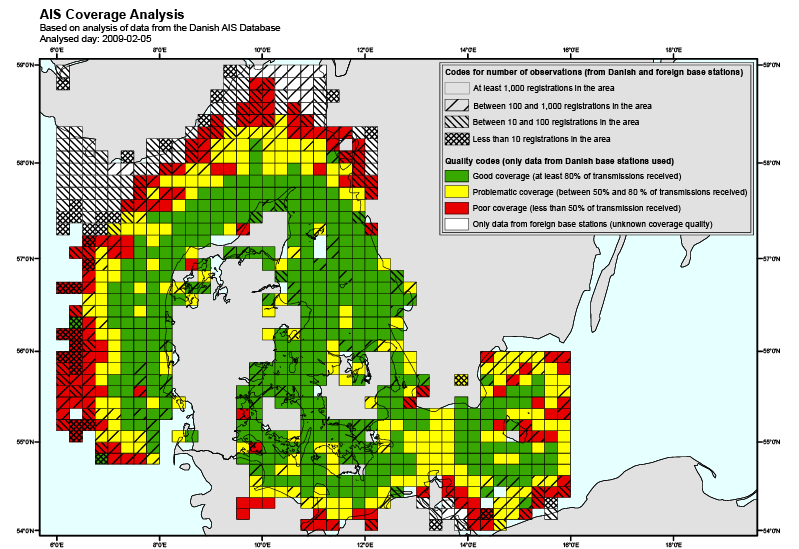
\includegraphics[width=0.8\textwidth]{02_figures/AIS_Coverage.png}
        \caption{Shore based AIS Coverage based on data from AIS database \cite{webaisdk.2023}}
        \label{fig:aiscoverage}
\end{figure}

In its initial state, the dataset contains 7453 data points which described the journey of the ship in one year. The initial data points represented all navigational statuses of the ship, which include ``mooring'', ``anchoring'' and ``underway using engine''. This is observed in the histogram for the SOG \Cref{fig:anomalies_sog_curspeed}.\\ 

To ensure the dataset accurately reflects the ship's operational status under steady conditions, a threshold for SOG is implemented. While variations in SOG can arise from changing sea conditions, they can also result from deliberate speed reduction during port departures or arrivals. Thus, any data points with SOG below 5 knots, which is indicative of manoeuvring, are removed \bcitep{Abebe.2020,Yan.2020}. Following this filtering step, the dataset size notably decreases from 7453 data points to 3828 data points. This reduction shows that approximately half of the original data points correspond to the ship's stationary activities.\\

% \begin{figure}
%     \centering
%         \includegraphics[width=0.8\textwidth]{02_figures/SassnitznoFilter.png}
%         \caption{Journey of the ship in a year}
%         \label{fig:YearJourney}
% \end{figure}
\begin{figure}[h!]
    \centering
        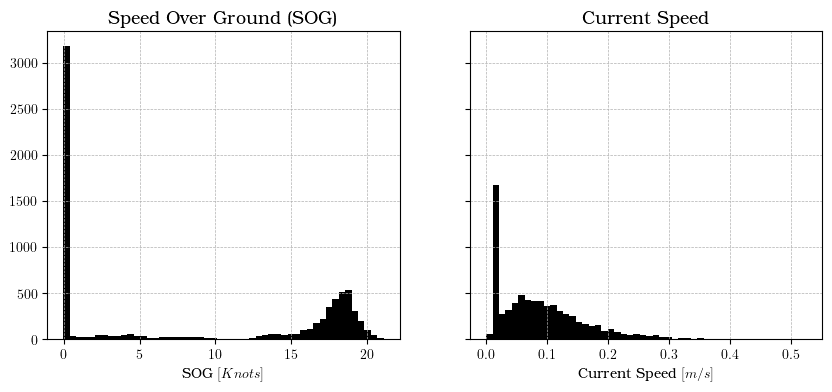
\includegraphics[width=0.9\textwidth]{02_figures/sog_curspeed_anomalies.png}
        \caption{Histogram plot of pre-filtered SOG and current speed}
        \label{fig:anomalies_sog_curspeed}
\end{figure}

Preliminary analysis reveals a potential source of error in data points representing current speed. Within the range of current speeds between 0.01 and 0.03 m/s, a distinct peak in data points is evident, as depicted in Figure \Cref{fig:anomalies_sog_curspeed}. This peak can be attributed to incomplete information regarding northward and eastward current speed in certain data points within the provided dataset. Consequently, a single random error value for the current speed is generated, leading to the observed peak in the histogram.\\

\begin{figure}[h]
    \centering
        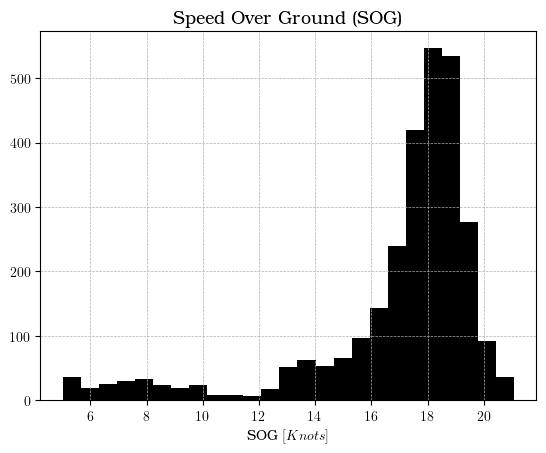
\includegraphics[width=0.6\textwidth]{02_figures/hist_init_sog_postfilter.png}
        \caption{Histogram plot of SOG after threshold}
        \label{fig:SOG_greater_five}
\end{figure}

To address the presence of missing values, the \texttt{KNNImputer} feature from \scikit/ is utilized to impute the missing values for eastward current and northward current. This step is essential as the modelling package provided by \scikit/ cannot handle instances with missing values. During the imputation process, the missing values for each sample are filled in using the mean value of the nearest neighbours found within the training dataset \bcitep{FabianPedregosa.2011}. The choice of using a k-nearest neighbour imputation strategy is appropriate, as it aims to capture the weather conditions within the vicinity of the missing values. Once the missing values for the northward and southward currents have been imputed, the current speed for these instances will be re-calculated. This k-nearest neighbour imputation approach is also extended to other weather features that contain missing values, specifically the \texttt{NaN} values.\\

\subsection{Feature Selection}\label{sec:feature_select}

In order to choose suitable features for the model, the correlation among different features is initially examined. Feature selection is essential to simplify the model and consequently reduce computational expenses during the training phase. The process of feature selection follows a statistical technique known as the High Correlation Filter, as proposed by \bcitet{Abebe.2020}. This method treats pairs of features with correlation coefficients exceeding 0.7 as a single entity. Nonetheless, the process of selecting highly correlated features must align with established physical principles. Hence, feature selection in this study is predominantly guided by physical reasoning, and this principle takes precedence over purely statistical considerations.\\

From AIS data, the information on \emph{time, latitude, longitude, width and length} are excluded, considering that time, latitude and longitude only describe the location of the ship at a particular position and the width and length of the ship are constant dimensions. As elaborated in \Cref{sec:weather_definition}, certain features like \emph{combined wind wave swell height, swell height, maximum wave height,} and \emph{wind wave height} are interconnected by physical relationships. The combined wind wave swell height corresponds to the significant wave height $H_{1/3}$, which is mathematically described by \Cref{eqn:H_sig_root}. Furthermore, \Cref{eqn:H_s_and_Tp} illustrates how the significant wave height serves to identify whether the sea is dominated by swell or wind-generated waves.\\

\begin{table}
    \footnotesize
    \centering
    % \resizebox {\textwidth}{!}
    {\begin{tabular}{ p{8cm}c }
    \hline
    \multicolumn{2}{l}{\textbf{Training Label}}\\
    \hline
    SOG [Knots] & {\tt sog} \\
    \hline
    \multicolumn{2}{l}{\textbf{Training Features}}\\
    \hline
    COG [°] & {\tt cog}  \\
    Heading [°] & {\tt heading}  \\
    Draught [m] & {\tt draught} \\
    Wind Speed [m/s] & {\tt windspeed} \\
    Air Temperature Above Oceans [K] & {\tt oceantemperature} \\
    % Maximum Wave Height [m] & {\tt waveheight} \\
    Wave Period [s] & {\tt waveperiod}\\
    Sea Surface Temperature [K] & {\tt surftemp}\\
    Combined Wind Wave Swell Height [m] &  {\tt windwaveswellheight} \\
    Current Speed [m/s] & {\tt curspeed} \\
    True Wind Direction [°] & {\tt truewinddir}  \\
    True Current Direction [°] & {\tt truecurrentdir} \\
    True Wave Direction [°] & {\tt truewavedir} \\
    \hline
    \end{tabular}}
\caption{Structure of training dataset}\label{tbl:struct_train_final}
\end{table}

Hence, it is evident that retaining the significant wave height is essential for the model, given that various wave properties can be deduced from it. Features like swell height, wind wave height, and maximum wave height will be excluded, as they can be determined from the significant wave height $H_{1/3}$. This choice is also substantiated by statistical analysis using the high correlation filter method. As depicted in \Cref{fig:heatmap_ovr}, high correlations exist among $H_{1/3}$, swell height, wind wave height, and maximum wave height.\\

\begin{figure}[h!]
    \centering
    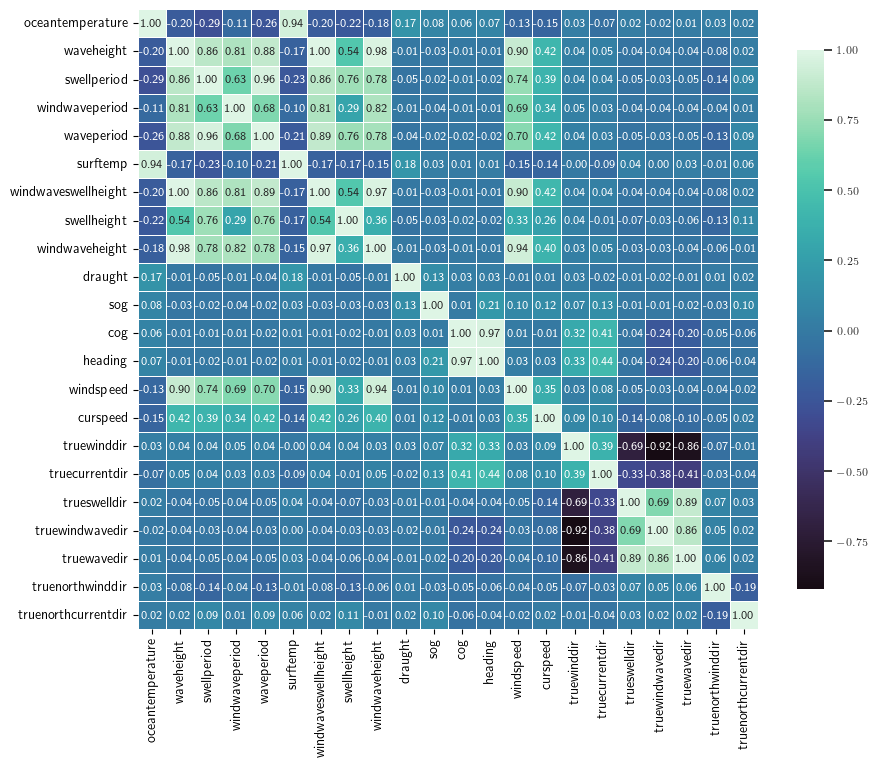
\includegraphics[width=.9\linewidth,height=.9\textheight,keepaspectratio]{02_figures/heatmap_corr_ovr.png}
    \caption{Correlation Heat Map}
    \label{fig:heatmap_ovr}
\end{figure}

\Cref{fig:heatmap_ovr} illustrates a significant correlation between wave period, swell period, and wind wave period. As outlined in \Cref{sec:weather_definition}, the sea state's description involves the significant height $H_{1/3}$ and spectral peak $\text{T}_p$ through the Torsethaugen peak method \bcitep{K.Torsethaugen.2004}. Consequently, the features swell period and wind wave period will be omitted, as they primarily differentiate whether the sea is influenced by swell or wind. However, the wave period feature will be retained. Therefore, the attributes ``true wind wave direction'' and ``true swell direction'' will also be disregarded since the features accounting for their magnitude have been removed.\\

In a statistical sense, heading and COG are significantly correlated, yet both features are retained due to their representation of distinct ship parameters. Course Over Ground (COG) signifies the ship's course heading while heading signifies the ship's actual heading at a specific time point. A similar rationale applies to the relationship between air temperature above the ocean and sea surface temperature. Air temperature above oceans represents wind temperature, whereas sea surface temperature reflects the temperature of the water surface. Following this principle, 5 features from the AIS data and 11 features from the weather data are omitted through feature selection. For predicting ship speed, SOG is selected as the target label for model training. The remaining attributes are chosen as training features. This is summarised in \Cref{tbl:struct_train_final}.\\

% \begin{table}
%     \footnotesize
%     \centering
%     % \resizebox {\textwidth}{!}
%     {\begin{tabular}{ p{8cm}c }
%     \hline
%     \multicolumn{2}{l}{\textbf{Training Label}}\\
%     \hline
%     SOG [Knots] & {\tt sog} \\
%     \hline
%     \multicolumn{2}{l}{\textbf{Training Features}}\\
%     \hline
%     COG [°] & {\tt cog}  \\
%     Heading [°] & {\tt heading}  \\
%     Draught [m] & {\tt draught} \\
%     Wind Speed [m/s] & {\tt windspeed} \\
%     Air Temperature Above Oceans [K] & {\tt oceantemperature} \\
%     % Maximum Wave Height [m] & {\tt waveheight} \\
%     Wave Period [s] & {\tt waveperiod}\\
%     Sea Surface Temperature [K] & {\tt surftemp}\\
%     Combined Wind Wave Swell Height [m] &  {\tt windwaveswellheight} \\
%     Current Speed [m/s] & {\tt curspeed} \\
%     True Wind Direction [°] & {\tt truewinddir}  \\
%     True Current Direction [°] & {\tt truecurrentdir} \\
%     True Wave Direction [°] & {\tt truewavedir} \\
%     \hline
%     \end{tabular}}
% \caption{Structure of training dataset}\label{tbl:struct_train_final}
% \end{table}

\begin{table}
    \footnotesize
    \centering
    % \resizebox {\textwidth}{!}
    {\begin{tabular}{ p{0.23\linewidth} c c c c c c c c }
    \hline
    Features & Count & Mean & Std. & Min & 25\% & 50\% & 75\% & Max \\
    \hline
    \textbf{{\tt sog}} & 2871 & 16.91 & 3.18 & 5.03 & 16.56 & 17.94 & 18.72 & 21.07\\
    \hline
    {\tt cog} & 2871 & 196.47 & 85.93&	69.77 & 102.58& 188.01& 282.26& 355.07\\ 
    {\tt heading} & 2871 & 187.88&	88.47&	67.90&	100.86&	124.65&	279.19&	355.07\\
    {\tt draught} & 2871 &5.22& 0.18& 4.74& 5.11& 5.28& 5.38&5.67\\
    {\tt windspeed} & 2871 & 6.42 & 2.97 & 0.25 & 4.13 & 6.15 &	8.36 & 16.01\\
    {\tt oceantemperature}\tablefootnote{Air temperature above oceans}& 2871 & 282.71 & 6.49 & 264.08& 277.13& 282.64& 288.82& 296.83 \\
    {\tt waveperiod} & 2871& 3.66& 0.82& 1.86& 3.07& 3.57& 4.14& 7.05\\
    {\tt surftemp}\tablefootnote{Sea Surface Temperature}&2871 &283.40& 5.73& 273.05& 278.13& 282.83& 288.86 &294.75\\
    {\tt windwaveswellheight}\tablefootnote{Significant wave height}  &  2871 & 0.75 & 0.51 & 0.07 &0.38 &	0.64 &	0.95 &  3.70  \\
    {\tt curspeed} & 2871 &0.10& 0.07& 0.00 & 0.05& 0.08 & 0.13 & 0.53\\
    {\tt truewinddir} & 2871 & 87.14 & 55.96 &	0.00 & 34.19 &	84.79 & 140.58 & 179.77	\\
    {\tt truecurrentdir} & 2871 & 89.15 & 57.53 & 0.25 & 31.01 & 86.78 & 143.32 & 179.99 \\
    {\tt truewavedir} & 2871 & 91.74 & 55.53& 0.13& 39.12 & 92.28 & 143.33 & 179.92 \\
    \hline
    \end{tabular}}
\caption{Descriptive statistics of preprocessed dataset}\label{tbl:dataset_descriptive_pretraining}
\end{table}

\begin{figure}
    \centering
    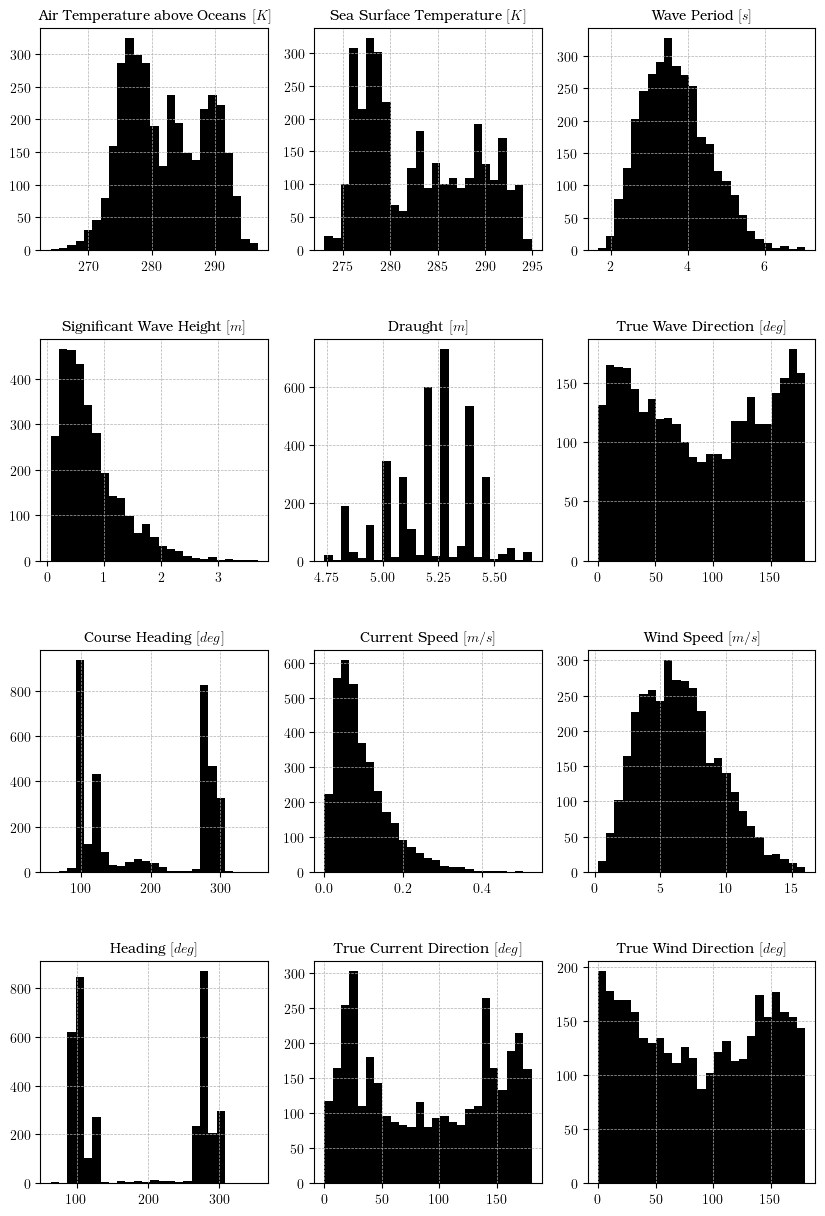
\includegraphics[width=.9\linewidth]{02_figures/hist_init_preprocessing.png}
    \caption{Histogram of training features}
    \label{fig:hist_training_ftr_label}
\end{figure}

\section{Black Box Modelling}\label{sec:BBM_modelling}

In this section, the modelling of ship speed based on SOG using the selected features will be conducted employing a tree-based regressor model. The considered tree-based regressor models comprise the decision tree regressor (DTR), random forest regressor (RFR), and extra-tree regressor (ETR). Additionally, to establish a benchmark, the tree-based models are compared against multiple linear regressors (MLR). The dataset is divided into training and test datasets with a ratio of 75:25 for training and testing, respectively. This results in 2871 data points for training and 957 data points for testing. To facilitate robust evaluation, the training dataset is subjected to 10-fold splitting. The hyperparameters of the tree-based regressors will be systematically fine-tuned through iterative processes until no further improvement to the model's performance can be achieved.\\


\subsection{Performance Metrics for Validation}\label{sec:perf_metrics}

To obtain a meaningful assessment of the model's performance and its precision, a cross-validation technique known as k-folding will be employed. K-fold cross-validation involves dividing the training set into k subsets, referred to as folds. Subsequently, the model will undergo k training iterations, using k-1 subsets for training and the remaining subset for validation. This process is visually depicted in Figure \ref{fig:kfold}. During each iteration, the model's performance will be evaluated using various metrics, including the \textbf{Coefficient of Determination ($R^2$), Explained Variance (EV), Mean Absolute Error (MAE), Root Mean Square Error (RMSE), Median Absolute Deviation (MAD), and Mean Absolute Percentage Error (MAPE)}. The outcomes from each iteration will be averaged, enabling an assessment of the model's precision, which can be further understood through the standard deviation. The application of k-fold cross-validation aids in evaluating the model's robustness across different datasets. The characteristics of each performance metric will be discussed in the subsequent sections.\\

\begin{figure}
    \centering
    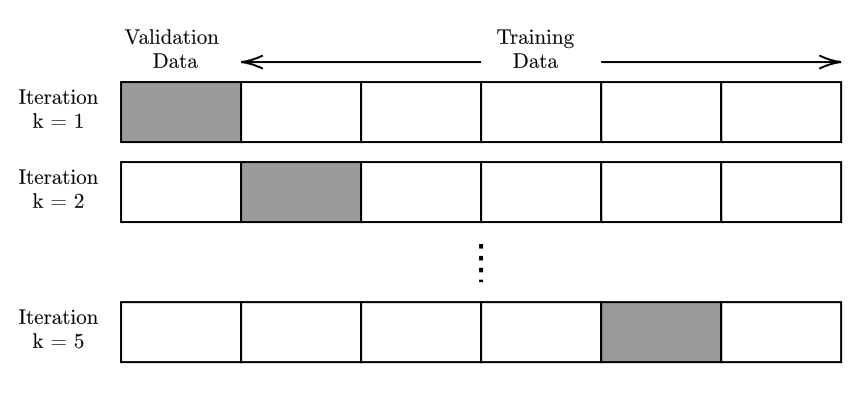
\includegraphics[width=.85\textwidth]{02_figures/kfold.png}
    \caption{Visual illustration of k-folding, Grey shaded box represents the validation data while white box represents the training data}
    \label{fig:kfold}
\end{figure}

\subsubsection*{Coefficient of Determination ({$R^2$})}\label{sec:rsquared}

The coefficient of determination $R^2$ gives a measure on prediction quality, $R^2$ quantifies the ability of the regression model to approximate the actual values. $R^2 $ is defined by \Cref{eqn:rsquared}, where $y$ represents true target output, $\hat{y}$ represents the predictor output and $\overline{y}$ represents the mean. $R^2$ score range between 0 and 1, higher values i.e. $R^2 \rightarrow 1$ indicate better model fit and a score of 1 indicates perfect prediction.\\

\begin{equation}\label{eqn:rsquared}
    R^2(y,\hat{y}) = 1 - \frac{\sum_{i = 1}^{n} (y_{\text{i}} - \hat{y}_{\text{i}} )^2 }{\sum_{i = 1}^{n} (y_{\text{i}} - \overline{y}_{\text{i}})^2} \quad \textbf{where} \quad \overline{y} = \frac{1}{n}\sum_{1}^{n} y_\text{i}
\end{equation}

\subsubsection*{Explained Variance (EV)}\label{sec:expVar}

Explained variance indicates how well a model can capture variance from a dataset. It is defined by \Cref{eqn:expVar}, where $\sigma_x$ represents the standard deviation of parameter $x$. EV score range between 0 and 1, where the best score of $EV = 1$ can be obtained if $\sigma^2_{(y-\hat{y})} \rightarrow 0$.\\  

\begin{equation}\label{eqn:expVar}
    EV(y,\hat{y}) = 1 - \frac{\sigma^2_{(y-\hat{y})}}{\sigma^2_{y}}
\end{equation}

\subsubsection*{Mean Absolute Error (MAE)}\label{sec:MAE}

MAE indicated the expected value of absolute ($L^1$ norm) error, and it can be calculated by:

\begin{equation}\label{eqn:MAE}
    MAE(y,\hat{y}) = \frac{1}{n}\sum_{i=1}^{n} |y_{\text{i}} - \hat{y}_{\text{i}}| 
\end{equation}

\subsubsection*{Root Mean Square Error (RMSE)}\label{sec:RMSE}

The RMSE describe the expected value of quadratic error. RMSE place a large penalty on large deviations between true and estimated values and for this reason, it can be used as a metric to indicate model performance against outliers. The ideal score is observed when $\text{RMSE} \rightarrow 0$. RMSE can be considered an absolute measure of model fitness. Omitting the root term, RMSE becomes MSE, which is the loss function of \Cref{eqn:costfun} that is used to determine the most optimal split in a regression decision tree.\\

\begin{equation}\label{eqn:RMSE}
    RMSE(y,\hat{y}) = \sqrt{\frac{1}{n}\sum_{i=1}^{n} (y_{\text{i}} - \hat{y}_{\text{i}})^2} 
\end{equation}

\subsubsection*{Median Absolute Deviation (MAD)}\label{sec:MAD} 

MAD is a performance metric that considers the median of the absolute errors. It is robust to outlier as it only considers median performance

\begin{equation}\label{eqn:MAD}
    MAD(y,\hat{y}) =  \text{median} (|y_{\text{1}} - \hat{y}_{\text{1}}|,\dots,|y_{\text{i}} - \hat{y}_{\text{i}}|)
\end{equation}

\subsubsection*{Mean Absolute Percentage Error (MAPE)}

Is an alternative to MAE, which provide easier interpretation, the result of MAPE can be interpreted according to \Cref{eqn:MAPE} \bcitep{MontanoMoreno.2013}. The usage of MAPE in model evaluation is to get an initial estimate, as MAPE comes with some drawbacks such as instability when $y_i = 0$ and it may lead to biased forecast \bcitep{Gkerekos.2019}. As such, the evaluation of the model performance will be mainly based on MAE and RMSE.    

\begin{equation}\label{eqn:MAPE}
    MAPE(y,\hat{y}) = \frac{1}{n}\sum_{i=1}^{n} \biggl|\frac{y_{\text{i}} - \hat{y}_{\text{i}}}{y_i}\biggr| \cdot 100\%  \quad \textbf{with} \quad \begin{array}{l c}
        \text{MAPE} & \text{Interpretation}\\
        \hline
        < 10 & \text{Highly accurate forecasting} \\
        10-20 & \text{Good Forecasting} \\
        20-50 & \text{Reasonable forecasting}\\
        > 50 & \text{Inaccurate forecasting} \\
        \hline
    \end{array}
\end{equation}

\subsection{Model Hyperparameter Optimisation}\label{sec:hpo}

The subject of parameter tuning was briefly discussed in \Cref{sec:dt_theo}. In \Cref{sec:dt_theo} parameter tuning was applied to the decision tree regressor to avoid overfitting by changing the minimum amount of samples a leaf node has. This example implies that altering the model hyperparameter will affect the model performance. However, the optimisation of the hyperparameter cannot be performed \emph{a priori} and as such iterative process will be performed until the best hyperparameter value is found.\\ 

\begin{table}[ht]
    \scriptsize
    \centering
    % \resizebox {\textwidth}{!}
    {\begin{tabular}{ p{0.33\textwidth}p{3cm}p{3cm}p{3cm}  }
    \hline
    \multicolumn{1}{c}{\textbf{Model}} & \multicolumn{1}{c}{\textbf{Decision Tree}}  & \multicolumn{1}{c} {\textbf{Random Forest}} & \multicolumn{1}{c}{\textbf{Extra-Trees}}\\
    \hline
    Number of trees & \multicolumn{1}{c}{1} & \multicolumn{1}{c}{Many} & \multicolumn{1}{c}{Many}\\
    Features considered for split at each node &   \multicolumn{1}{c}{All features}  & \multicolumn{1}{c}{Random subset of features} & \multicolumn{1}{c}{Random subset of features} \\
    Bootstrapping & \multicolumn{1}{c}{Not applied} & \multicolumn{1}{c}{Yes} & \multicolumn{1}{c}{No}\\
    Split Rule  & \multicolumn{1}{c}{Best split} & \multicolumn{1}{c}{Best split}& \multicolumn{1}{c}{Random split}\\
    \hline
    \end{tabular}}
\caption{Comparison of tree-based model from \Cref{sec:tree_intro}}\label{tbl:table_trees}
\end{table}

\scikit/ offers {\tt GridSearchCV} and {\tt RandomizedSearchCV} to help search for the most optimal hyperparameter. Both solutions operate with similar principle: The selected hyperparameters to be tuned with their value range are evaluated using cross-validation to evaluate the best possible combination between the selected hyperparameters. The difference between {\tt GridSearchCV} and {\tt RandomizedSearchCV} lies in how it searches for the best value for the selected hyperparameters: {\tt GridSearchCV} involves the construction of grids containing all possible combinations of hyperparameter value in a specified range.{\tt RandomizedSearchCV} randomly samples hyperparameter values. The exhaustive nature of {\tt GridSearchCV} means that it is computationally costly to perform, especially when there are multiple hyperparameters to be considered and the value search space is large. {\tt RandomizedSearchCV} gives more control to computing budget by setting the number of iterations and usually produces more accurate results than {\tt GridSearchCV} approach. \bcitep{Geron.2019,J.Bergstra.2012}. \\

To address this issue, the {\tt RandomizedSearchCV} technique will be applied to identify the optimal hyperparameters. However, it's important to note that a lack of \emph{a priori} knowledge regarding hyperparameter values remains a challenge. Despite the ability of {\tt RandomizedSearchCV} to manage computational resources, obtaining the best hyperparameter values can still demand a significant amount of time. This could potentially lead to spending computational resources on searches within unpromising search spaces. Therefore, an initial investigation into the impact of each hyperparameter on model performance will be conducted. This preliminary exploration aims to provide a clearer understanding of which search spaces should be considered during the subsequent hyperparameter optimization process. In the forthcoming subsections, the influence of tunable hyperparameters within the tree-based models from \scikit/ will be examined. This exploration seeks to establish baseline values for the search space. Throughout this analysis, MAE will serve as the chosen performance metric. The hyperparameter optimization pursued within this thesis is aimed towards minimising prediction errors.\\

\subsubsection*{Number of features}\label{sec:max_features}

Defined with default value as {\tt max\_features=None} in \scikit/. This hyperparameter controls the number of features to be considered when looking for the best split, the default {\tt None} option means it will consider all features. This parameter tuning is available for Decision Tree Regressor, Random Forest Regressor and Extra-Tree Regressor. Initial exploration indicated Random Forest Regressor and Extra Tree Regressor benefit from considering more features. Decision Tree Regressor also benefits from considering all features for determining the split.\\ 

\begin{figure}[h]
    \centering
        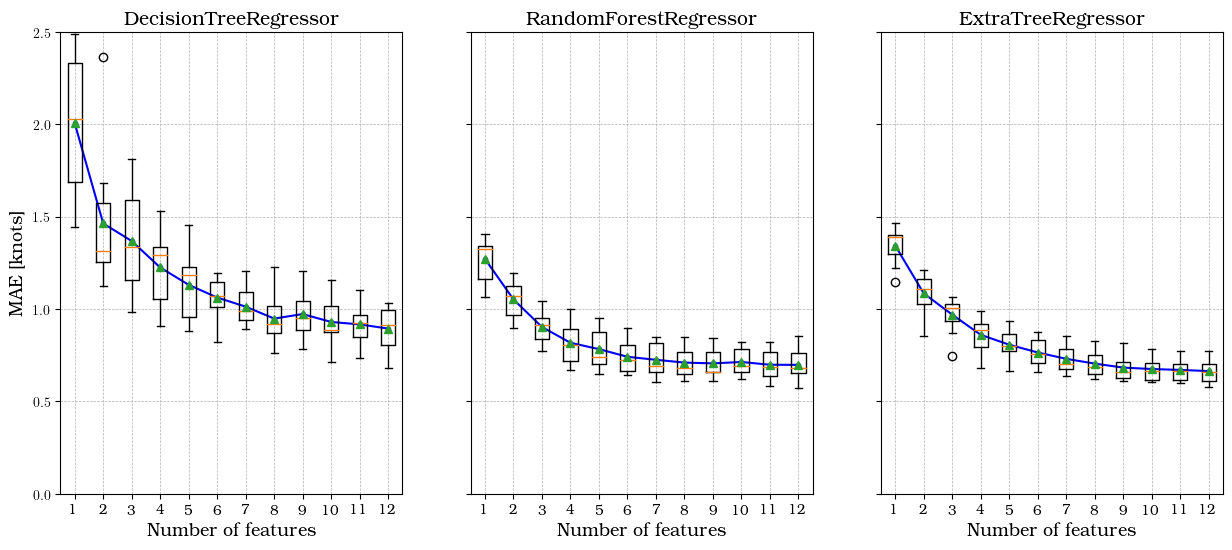
\includegraphics[width=.85\textwidth]{02_figures/hpo_n_features_mae.png}
        \caption{Hyperparameter tuning of {\tt max\_features}}
        \label{fig:hpo_n_features}
\end{figure}

\subsubsection*{Minimum samples to split a node}\label{sec:min_samples_split}

Defined with default value as {\tt min\_samples\_split=2} in \scikit/. This hyperparameter controls the minimum number of samples i.e. data points required to split a node. The default value of {\tt 2} is the least number of samples required to split a node i.e. 1 sample is split to the left and right branches respectively. The plot at \Cref{fig:hpo_min_samples_leaf} indicates that tuning this hyperparameter will not have any major impact on any model's performance.\\
\begin{figure}[h]
    \centering
        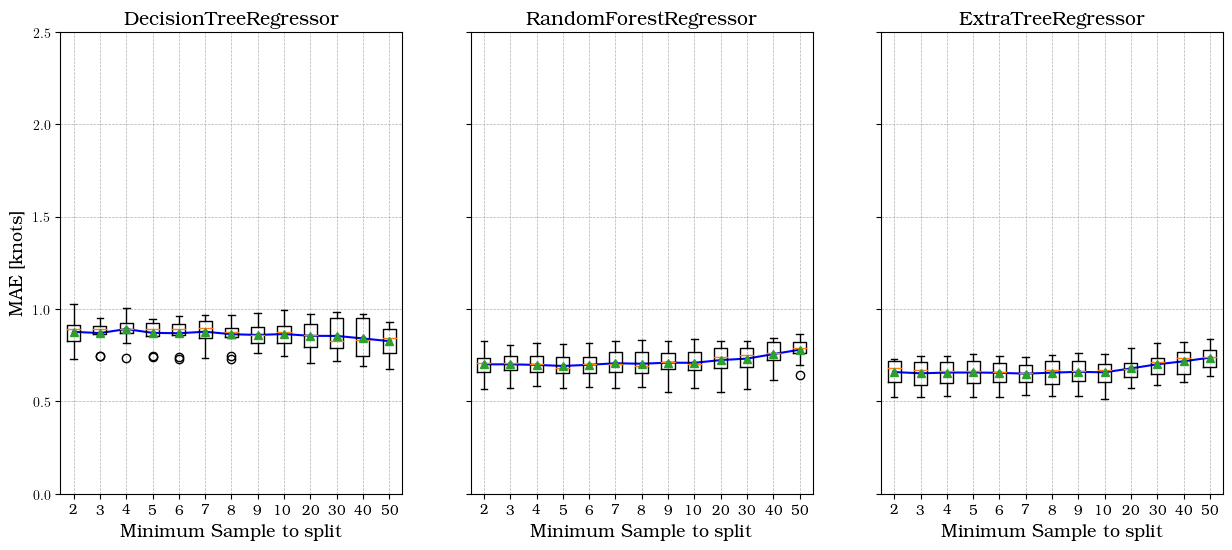
\includegraphics[width=.85\textwidth]{02_figures/hpo_min_samples_split_mae.png}
        \caption{Hyperparameter tuning of {\tt min\_samples\_split}}
        \label{fig:hpo_min_samples_split}
\end{figure}

\subsubsection*{Number of sample in a leaf node}\label{sec:min_samples_leaf}

Defined with default value as {\tt min\_samples\_leaf=1} in \scikit/. This parameter controls the number of samples required to be at the leaf node, where the split point will be considered if the leaf contains at least {\tt min\_samples\_leaf=n} training samples in each left and right branch. As shown in \Cref{fig:geron6_6}, tuning this hyperparameter to higher values helps to smoothen the model and avoid overfitting. However, this may lead to underfitting as the model is unable to capture the trend within the data. This is supported by the findings shown in \Cref{fig:hpo_min_samples_leaf}, the DTR benefits from regularisation at a certain breakeven point. But, after this breakeven point, the model's performance degrades. It is also observed that tuning this parameter will negatively impact RFR and ETR model's performance. 

\begin{figure}[h]
    \centering
        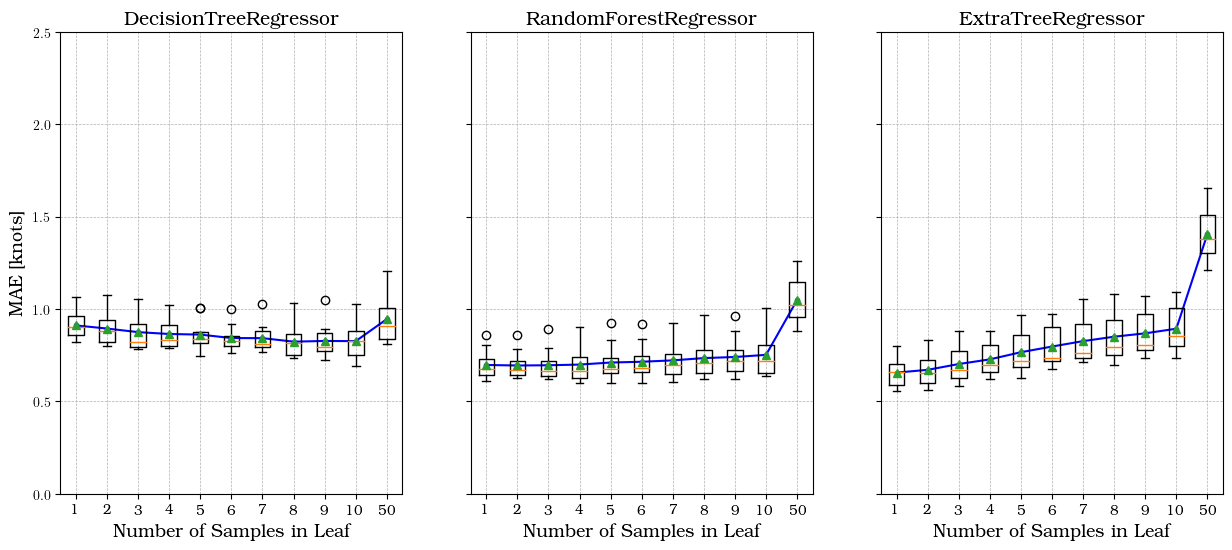
\includegraphics[width=.85\textwidth]{02_figures/hpo_min_samples_leaf_mae.png}
        \caption{Hyperparameter tuning of {\tt min\_samples\_leaf}}
        \label{fig:hpo_min_samples_leaf}
\end{figure}

\subsubsection*{Depth of Tree}\label{sec:max_depth}

Defined with default value as {\tt max\_depth=None} in \scikit/. This hyperparameter is defined as the count of nodes along a path from the root node to its parent node. Leaving it at {\tt max\_depth=None} means the tree will grow until all leaves are pure i.e. until minimum MSE is obtained or when the number of samples is less than the minimum number of samples required to split an internal node. Similar to {\tt min\_samples\_leaf}, DTR shows improvement until a certain breakeven point. RFR performance seems to stabilise at a certain depth while ETR benefits from allowing full growth of the tree. It can also be observed that the models' performance are identical for {\tt max\_depth=1}, which is evident as shown in \Cref{fig:hpo_max_depth}  

\begin{figure}[h]
    \centering
        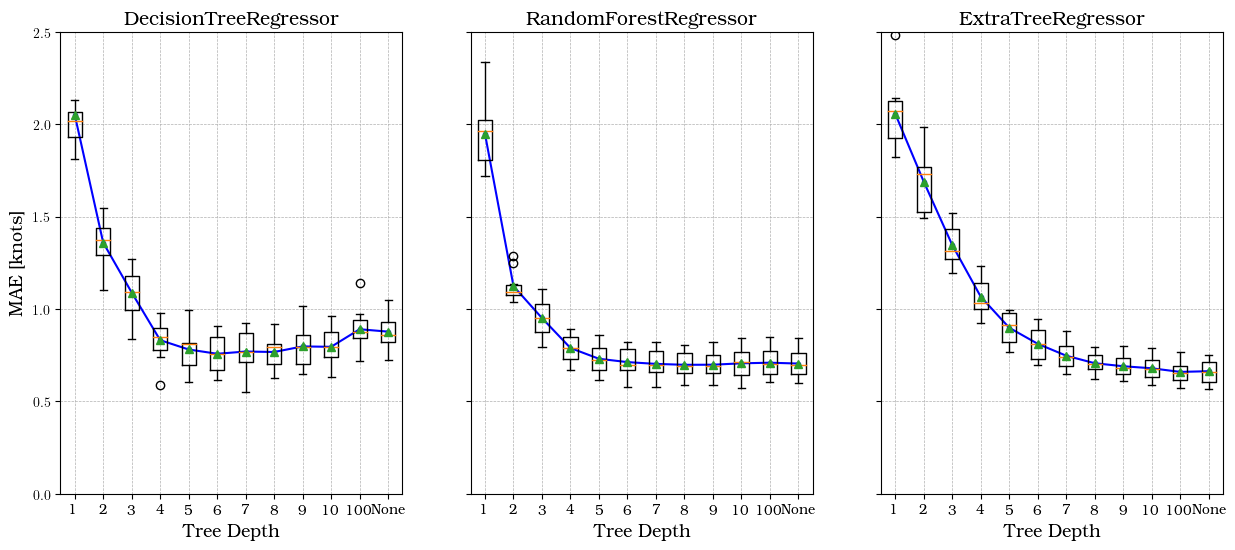
\includegraphics[width=.85\textwidth]{02_figures/hpo_max_depth_mae.png}
        \caption{Hyperparameter tuning of {\tt max\_depth}}
        \label{fig:hpo_max_depth}
\end{figure}

\subsubsection*{Number of Trees}\label{sec:n_estimators}

Defined with default value as {\tt n\_estimators=100}. This hyperparameter controls the amount of trees i.e. predictors in a forest. Tuning the number of trees will affect the training time, and it is only available to RFR and ETR. The default value seems to yield a satisfactory result, as the performance for both RFR and ETR stabilise after in this case stabilise after 100 trees, as seen in \Cref{fig:hpo_n_features}.
\begin{figure}[h]
    \centering
        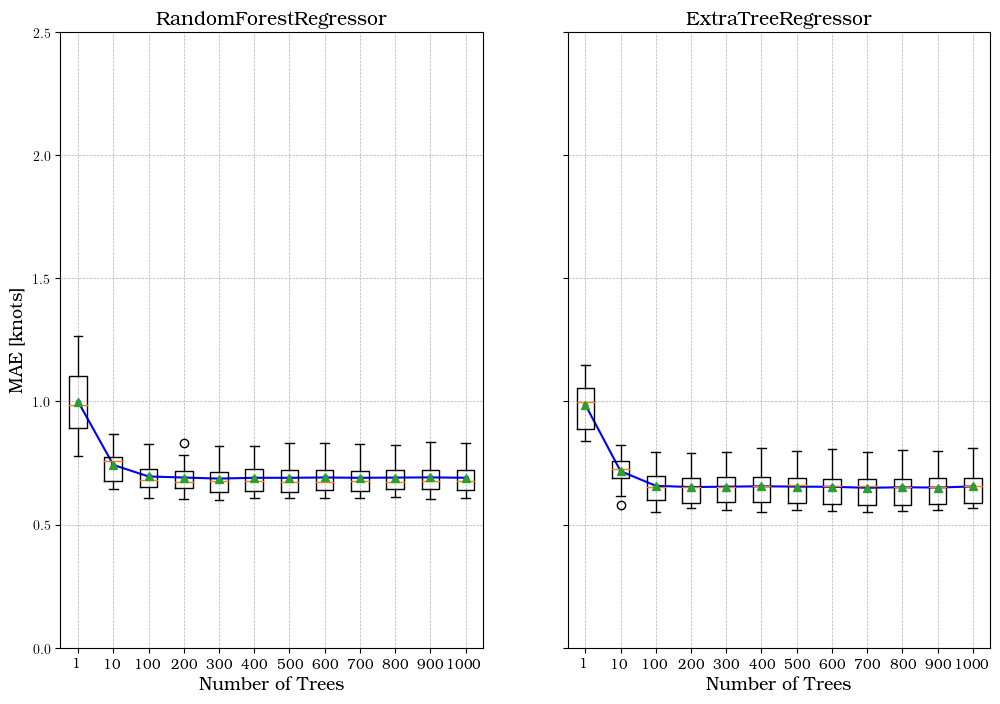
\includegraphics[width=.6\textwidth]{02_figures/hpo_n_estimators_mae.png}
        \caption{Hyperparameter tuning of {\tt n\_estimators}}
        \label{fig:n_estimators}
\end{figure}

\section{White Box Modelling}\label{sec:WBM_modelling}

This section involves the integration of the predicted SOG from the BBM into the WBM for the estimation of bunker fuel consumption (FOC). The Holtrop-Mennen approximation method will be employed to estimate the ship's encountered resistance, which will enable the determination of the total resistance crucial for calculating the power required for propulsion. However, it's worth noting that in the process of resistance calculation, certain form coefficients and ship parameters may not be readily available and could necessitate assumptions based on existing literature. Such assumptions will be explicitly indicated throughout this section. Subsequently, the resulting brake power $P_B$ will be plotted against the STW $v_S$ to generate a power-speed curve model. This model offers an alternative approach for estimating the FOC, representing the energy expended during a specific voyage.

\subsection{Calculation of Total Resistance}\label{sec:Rtot_calc_method}

The formula used to calculate total resistance $R_{TOTAL}$ in this section is presented in \Cref{sec:holtrop_mennen_calc} with the principle dimension of the ship which was given in \Cref{tbl:Hammershus_Data}. Some assumptions are made for the sea state and the values of some form coefficients are calculated based on empirical formulas presented in \Cref{sec:Ship_design_param}. In this case study, Holtrop-Mennen method can be used as it fulfils the condition set in \Cref{eqn:holtrop_cond}:
\begin{equation}
    \label{eqn:holtrop_cond_fulfill}
    % \begin{multlined}
    \begin{gathered}
        Fr = 0.2417  \leqslant 0.45 \\
        0.55 \leqslant C_P = 0.6707 \leqslant 0.85 \\
        3.9 \leqslant \frac{L}{B} = 5.91 \leqslant 9.5
    \end{gathered}
    % \end{multlined}
\end{equation}

The calculations of resistance are dynamics as the Froude number $Fr$ is based on $v_S$, and the design Froude number $Fr_{DESIGN}$ is used to check use cases for some equations.

\subsubsection*{Calculation of frictional resistance $R_F$}

For the calculation of the surface area of bare hull $S$, it is assumed that the aft has a U-shaped section. Then the appropriate $C_{stern}$ can be calculated to obtain the constant $c_{14}$ \Cref{eqn:c_14}. For the calculation of length of run $L_R$, approximation for $\ell_{CB}$ are made based on \Cref{eqn:lcb}. The constants $c_{14}$ and $L_R$ are used to calculate the form factor $1+k_1$ which will be used to calculate $R_F$.

\subsubsection*{Calculation of appendage resistance $R_{APP}$}

From known ship information and ship schematics shown in \Cref{fig:Hammershus_Pict}, it can be deducted that the ship consists of the following appendages:

\begin{itemize}
    \setlength\itemsep{0em}
    \item Two high-lift flap rudders
    \item Single centre skeg
    \item Twin shafts supported by two brackets
\end{itemize}

The assumptions for the appendage area are made by scaling the schematics to known measurements (e.g. the $L_{WL}$). From here, the appropriate $k_{2_i}$ constants for individual appendages will be selected from \Cref{tbl:k2i_values} to obtain the $(1+k_{2_i})_{eq}$ from \Cref{eqn:k2eq}.

\begin{table}[h]
    \footnotesize
    \centering
    % \resizebox {\textwidth}{!}
    {\begin{tabular}{ p{0.2\linewidth} c c}
    \hline
    Appendage type & Value & $(1+k_{2_i})$ \\
    \hline
    \multicolumn{2}{l}{\textbf{Two high-lift flap rudders}} & 3\\
    \hline
    $h_{\text{RUDDER}}$ & 4.06 $m$\\
    $B_{\text{RUDDER}}$ & 1.99 $m$\\
    $S_{\text{RUDDER}}$ & 16.16 $m^2$\\
    \hline
    \multicolumn{2}{l}{\textbf{Single centre skeg}} & 1.5\\
    \hline
    $h_{\text{SKEG}}$ & 4.41 $m$\\
    $B_{\text{SKEG}}$ & 26.23 $m$\\
    $S_{\text{SKEG}}$ & 115.67 $m^2$\\
    \hline
    \multicolumn{2}{l}{\textbf{Twin shafts supported by two brackets}} & 3\\
    \hline
    $D_{\text{SHAFT}}$ & 0.55 $m$\\
    $L_{\text{SHAFT}}$ & 13.54 $m$\\
    $S_{\text{SHAFT}}$ & 46.79 $m^2$\\
    \hline
    \multicolumn{1}{l}{\textbf{$S_{APP_{tot}}$}} & \textbf{178.62} $m^2$ \\
    \multicolumn{2}{l}{\textbf{$(1+k_{2_i})_{eq}$}} & \textbf{2.03} \\
    \end{tabular}}
\caption{Assumed appendage values}\label{tbl:assume_appendage_dimension}
\end{table}

Additionally, there are two bow thrusters installed with approximated diameter of $d_{TH}= 2.15 m$, from here, the constant $C_{D_TH}$ can be approximated using \Cref{eqn:R_th}. Hence, the appendage resistance $R_{APP}$ can be calculated using \Cref{eqn:R_app}.

\subsubsection*{Calculation of wave resistance $R_{W}$}

The calculation of wave resistance is based on the case for $Fr \leq 0.4$ using equation \Cref{eqn:R_w_low}. The estimation is done by adding the constants presented between \Cref{eqn:c_7} and \Cref{eqn:m4}. There are some use cases for some equations, which is summarised in \Cref{tbl:R_w_use_case}.

\begin{table}[h]
    \footnotesize
    \centering
    % \resizebox {\textwidth}{!}
    {\begin{tabular}{ p{0.2\linewidth} c c }
    \hline
    Constant & Use Case & Equation \\
    \hline
    $c_7$ &  $0.11 < \frac{B}{L_{WL}} \leq 0.25$ & \Cref{eqn:c_7} \\
    $c_{15}$ & $\frac{L_{WL}^2}{V} \leq 512$ & \Cref{eqn:c15} \\
    $c_{16}$ & $C_P \leq 0.8$ & \Cref{eqn:c16} \\
    $\lambda$ & $L_{WL} \leq 12$ & \Cref{eqn:lambda} \\
    \hline
    \end{tabular}}
\caption{Use case of constants for $R_W$}\label{tbl:R_w_use_case}
\end{table}

\subsubsection*{Calculation of bulbous bow resistance $R_B$}
The area $A_{BT}$ used to calculate is approximated based on \bcitet{Kracht.78} with:

\begin{equation}
    \label{eqn:A_BT}
    A_{BT} = 0.085 A_M
\end{equation}

For the height $h_B$, the upper limit of $h_B = 0.6T_{DESIGN}$ is selected, and it is assumed that $T_F = T_{DESIGN}$.

\subsubsection*{Calculation of (immersed) transom resistance $R_{TR}$}

Since the immersed transom area is unknown, \bcitet{Rakke2016} approximated the immersed transom area based on the correlation of ship dimension from the literature review of \bcitet{Holtrop.1982}:

\begin{equation}
    \label{eqn:A_TR}
    A_{TR} = 0.051 A_M
\end{equation}

This approximation must be used with caution as it is only based on case study of \bcitet{Holtrop.1982}. However, to author's best knowledge, there are no other literature that provide empirical estimation of $A_{TR}$. Therefore, this estimation will be selected in this case study. The selection for the value of constant $c_6$ is dependent on the value of $Fr_T$, which is a function of $v_S$. From there, the transom resistance can be calculated using \Cref{eqn:R_transom}

\subsubsection*{Calculation of correlation allowance resistance $R_A$}

The selection of constant $c_4$ in equation \Cref{eqn:c4} is based on the $T_F$, then the correlation resistance $R_A$ can be calculated using \Cref{eqn:R_a}.

\subsubsection*{Calculation of added resistance due to wind $R_{AA}$}

Two assumptions are made during the calculation of $R_{AA}$, since the information of lateral area $A_L$ and $A_F$ are not readily available, these values are assumed based on the dimension of similar ferry in the case study of \bcitet{Blendermann.1994}. It is assumed that the ferry has an $A_L$ of \textbf{2125.80} $m^2$ and $A_F$ of \textbf{325.30} $m^2$. From \Cref{tbl:BlendermannCoeff}, the case for ferry ship is taken to get the necessary constants for the calculation of $R_{AA}$. 

\subsubsection*{Calculation of added resistance due to wave $R_{AW}$ }

This part of the equation is relatively straightforward, $L_{BWL}$ will be approximated to about \textbf{43.75} m. The calculation of $R_{AWL}$ will be based on the data of significant wave height $H_{1/3}$ from the dataset.

\pagebreak

\subsection{Calculation of total efficiency $\eta_{TOT}$}\label{sec:eta_tot_method}

\subsubsection*{Calculation of open water efficiency $\eta_O$}

This value is approximated based on the line of the Wageningen series in \Cref{fig:breslin_open water efficiencies} \bcitep{Breslin.1994}. The case will be for ``Passenger ships and high-speed naval vessels''. Since the value of $C_{Th}$ is not available, the value of $\eta_O$ is approximated as \textbf{0.7}.

\subsubsection*{Calculation of hull efficiency $\eta_H$}

For the calculation of $\eta_H$, the value of the propeller diameter $D$ is approximated as \textbf{4 m}, which is based on the schematics of the ship shown in \Cref{fig:Hammershus_Pict}.

\subsubsection*{Calculation of relative rotative efficiency $\eta_R$}

The missing value required to compute \Cref{eqn: eta_rot_holtrop} is the pitch-diameter propeller ratio. This value will be estimated as $P/D =$ \textbf{1.135}, which is obtained from the work of \bcitet{Bertram.2000}.

\begin{figure}[h]
    \centering
        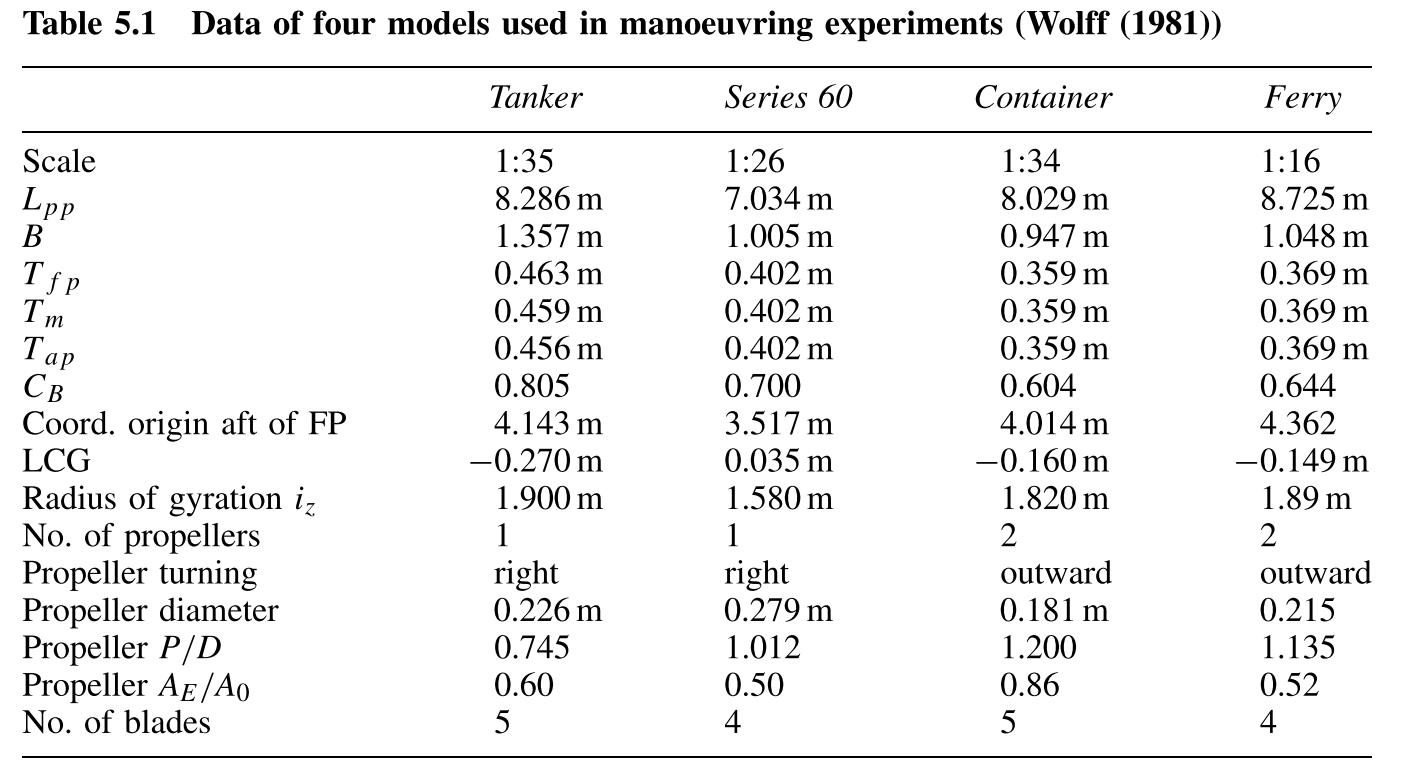
\includegraphics[width=.95\textwidth]{02_figures/betram_wolff_ratiomodel .jpg}
        \caption{Estimated value of propeller dimensions \bcitep{Bertram.2000}}
        \label{fig:betram_wolff_propellerdimensions}
\end{figure}

\subsubsection*{Calculation of shaft efficiency $\eta_S$}

The value of shaft efficiency is estimated as $\eta_S =$ \textbf{0.99} based on \bcitet{Diesel.2011} and \bcitet{Holtrop.1982}.

\subsection{Calculation of FOC}\label{sec:FOC_calc_method}

Once $R_{TOTAL}$ and $\eta_{TOTAL}$ are determined, the brake power of the ship, denoted as $P_B$, can be computed using Equation \ref{eqn:P_b}. The resultant $P_B$ values will then be graphed against the ship's STW ($v_S$), producing a power-speed curve. A regression line will be fitted to the data points on this curve. Since each BBM model generates distinct SOG predictions, the regression equation for the line signifies the characteristics of different BBM models. To assess the performance of each BBM, the regression models produced by each BBM will be compared against the regression model derived from actual data. This evaluation will gauge the predictive capabilities of each model. Subsequently, the FOC can be calculated using Equation \ref{eqn:FOC}. The specific fuel oil consumption (SFOC) information can be extracted from Table \ref{tbl:Hammershus_Data}. Without multiplication by the operational time $\tau_{OP}$, the fuel consumption in metric tons per hour ($T/h$) can be computed by dividing the value by $1 \times 10^6$.


\begin{table}
    \footnotesize
    \centering
    % \resizebox {\textwidth}{!}
    {\begin{tabular}{ p{0.1\linewidth} p{0.2\linewidth} p{0.6\linewidth}}
    \hline
    Parameter & Value & Remarks \\
    \hline
    $g$ & 9.805 $kg/ms^2$ \\
    $\rho_{sea}$ & 1025 $kg/m^3$ \\
    $\nu_{sea}$ & 0.00000118 $m^2/s$ \\
    $\rho_{air}$ & 1.25 $kg/m^3$ \\
    1 m/s & 1.9438 knots \\
    \hline
    \multicolumn{3}{l}{\textbf{Required Parameters for Holtrop-Mennen}}\\
    \hline
    $L_{WL}$ & 144.80 m & From \Cref{tbl:Hammershus_Data} \\
    $B$ & 24.50 m & From \Cref{tbl:Hammershus_Data} \\
    $T$ & 5.85 m & Assume $T_A = T_F = T$ for initial phase, otherwise use $T$ from dataset, also assume maximum draught \\
    $V$ & 13592.1413 $m^3$ & $V = C_B \cdot L_{WL} \cdot T_{MAX}$\\
    $Fr_{N}$ & 0.2417 & From \Cref{eqn:Froude_Number} \\
    $C_B$ & 0.6549 & From \Cref{eqn:Cb_Schneekluth}\\
    $C_M$ & 0.9764 & From \Cref{eqn:CM_jensen} \\
    $C_P$ & 0.6707 & From \Cref{eqn:cp_ratio}\\
    $C_{WP}$ & 0.7700 & From \Cref{eqn:cwp_Schneekluth}\\
    $\ell_{CB}$ & -0.0123 & \Cref{eqn:lcb}\\
    $A_{TR}$ & 7.3581 $m^2$ & \Cref{eqn:A_TR}\\
    $A_{BT}$ & 12.2634 $m^2$ &\Cref{eqn:A_BT}\\
    $h_B$ & 3.5100 m & Assume upper limit $h_{B} = 0.6T_F$\\
    $D$ & 4 m & Approximated from schematics \Cref{fig:Hammershus_Pict}\\
    $A_E / A_0$ & 1.135 & Value assumed from \Cref{fig:betram_wolff_propellerdimensions}\\
    $C_{stern}$ & 10 & Assume u-shaped section \Cref{eqn:c_14}\\
    \hline
    \multicolumn{3}{l}{\textbf{Optional Parameters for Holtrop-Mennen}}\\
    \hline
    $S$ & 3881.0231 $m^2$& approximated from \Cref{eqn:S_bh}\\
    $S_{APP}$ & $178.62 m^2$ & approximated from schematics \Cref{fig:Hammershus_Pict}\\
    $i_E$ & 21.6014° & \Cref{eqn:i_e}\\
    $d_{TH}$ & 2.15 m & Approximated from schematics \Cref{fig:Hammershus_Pict}\\
    \hline
    \end{tabular}}
\caption{Assumed values for power estimation}\label{tbl:assume_sea_constants}
\end{table}


